\title{Topics in Unsupervised Learning HW 1}
\author{Shir Hamawie \& Nadav Shoham}
\date{\today}

\documentclass[12pt]{article}
\usepackage{mathtools}
\usepackage{amsfonts}
\usepackage{relsize}
\usepackage[margin=1in]{geometry}
\usepackage{graphicx}
\usepackage{dblfloatfix}
\graphicspath{ {images/} }
\usepackage[font=normalsize,labelfont=bf]{caption}
\newtheorem{theorem}{Theorem}[section]
\newtheorem{corollary}{Corollary}[theorem]
\newtheorem{lemma}[theorem]{Lemma}
\newtheorem{definition}{Definition}[section]

\newcommand{\sigmastar}{\Sigma ^*}
\newcommand{\arrowstar}{\xrightarrow[]{*}}

\begin{document}
\maketitle
\begin{center}
\section*{Introduction}\label{sec:introduction}
\end{center}
In this assignment, we will implement the k-means and dc-dp-means clustering algorithms and evaluate their performance on different artificial datasets with different hyperparameters. We will compare the clustering results of the two algorithms and analyze their strengths and weaknesses.
\\
We will generate synthetic 2D data of N = 1000 points with different random states to see how our algorithms perform at different situations.
\\
\section*{Task 1}\label{sec:task-1}
In this task we implemented both algorithms and checked how they performed on the following generated data:

\begin{figure}[!h]
    \centering
    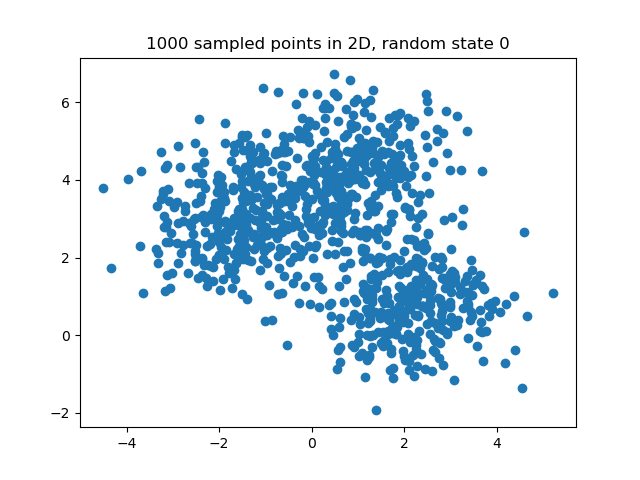
\includegraphics[scale=0.5]{images/data_0}\label{fig:figure2}
\end{figure}


The following images are our clustering results with k = 3 and l = 4:
\begin{figure}
    \begin{minipage}{0.5\textwidth}
    \centering
    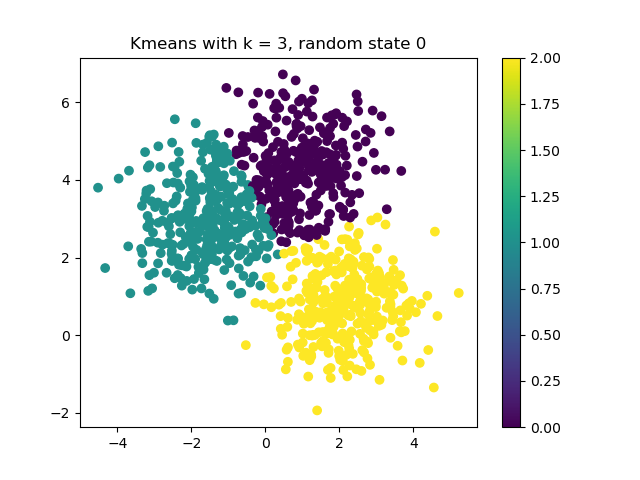
\includegraphics[scale=0.4]{images/task2_drs_rs0__k3}
    \caption{Kmeans}
    \end{minipage}
    \begin{minipage}{0.5\textwidth}
    \centering
    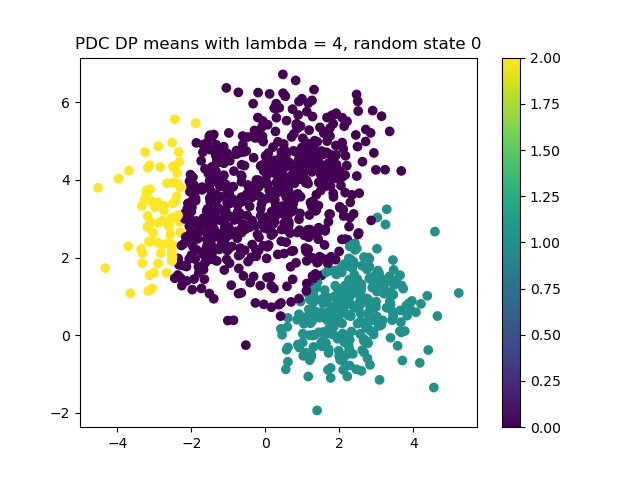
\includegraphics[scale=0.4]{images/task2_drs_rs0__l4}
    \caption{DC-DP Means}
    \end{minipage}\label{fig:figure}
\end{figure}
\newpage
We can see we got fairly reasonable clusters, where the kmeans clustering looks like better separation.
\\

\section*{Task 2}\label{sec:task-2}
The purpose of this part is to investigate the behavior of the algorithms in different scenarios and gain insights into their strengths and limitations.
First, we will test the algorithms on different datasets with different random states and compare the results.
Then we will test the algorithms on the same dataset with different hyper parameters and compare the results.
\subsection*{Different samples space initializations}
In this section, we will present the experimental results of applying the clustering algorithms on four more randomly
generated 2D datasets with varying degrees of complexity and structure.
We will evaluate the performance of the algorithms using the same hyper parameters as before and analyze the resulting clustering outputs.
\\
\begin{figure}[!h]
        \begin{minipage}{0.5\textwidth}
		\centering
		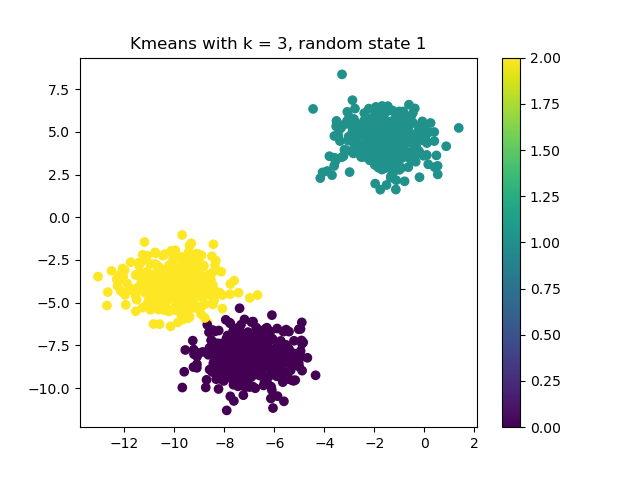
\includegraphics[scale=0.4]{images/task2_drs_rs1__k3}
	\end{minipage}
        \begin{minipage}{0.5\textwidth}
		\centering
		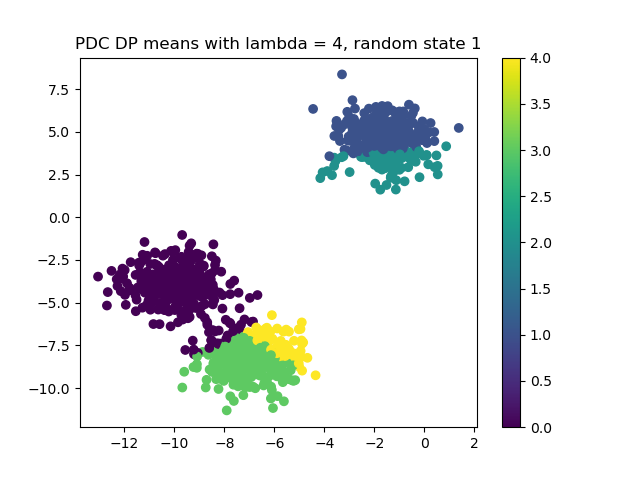
\includegraphics[scale=0.4]{images/task2_drs_rs1__l4}
	\end{minipage}\label{fig:figure3}
\end{figure}

\newpage
\begin{figure}
    \begin{minipage}{0.5\textwidth}
    \centering
    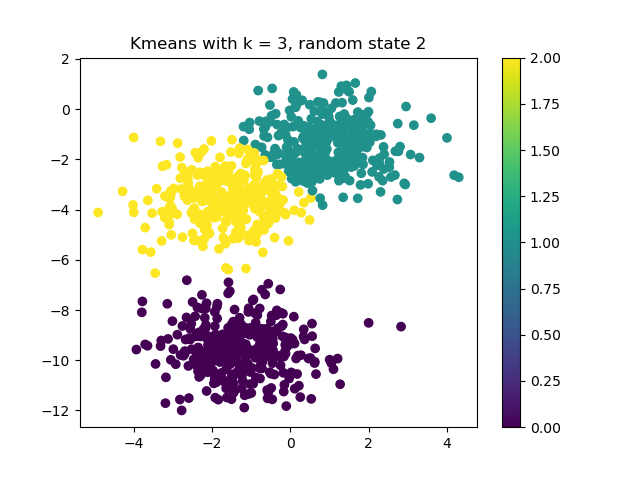
\includegraphics[scale=0.4]{images/task2_drs_rs2__k3}
    \end{minipage}
    \begin{minipage}{0.5\textwidth}
    \centering
    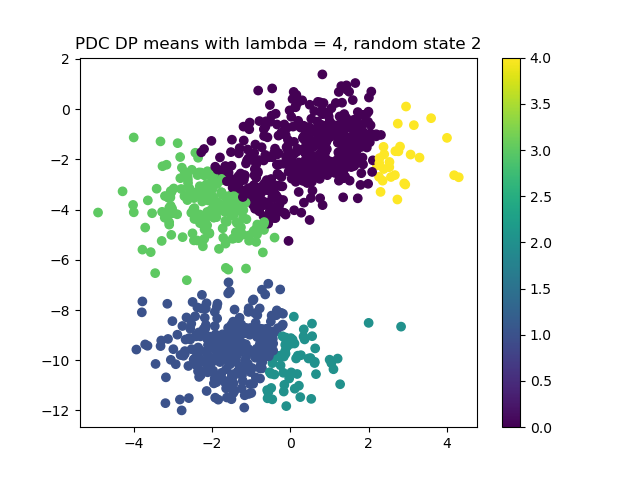
\includegraphics[scale=0.4]{images/task2_drs_rs2__l4}
    \end{minipage}
    \begin{minipage}{0.5\textwidth}
    \centering
    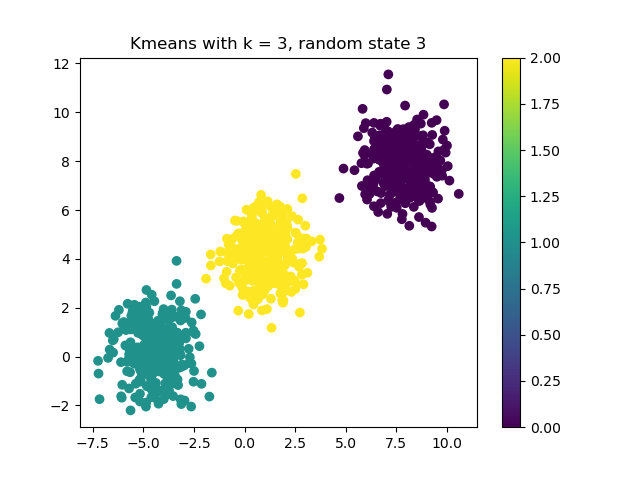
\includegraphics[scale=0.4]{images/task2_drs_rs3__k3}
    \end{minipage}
    \begin{minipage}{0.5\textwidth}
    \centering
    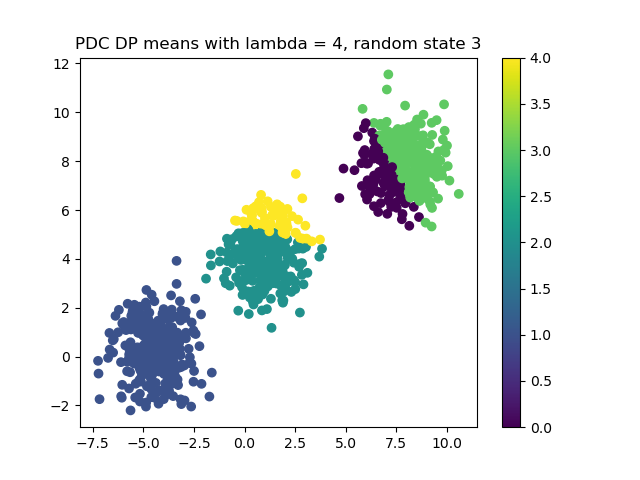
\includegraphics[scale=0.4]{images/task2_drs_rs3__l4}
    \end{minipage}
    \begin{minipage}{0.5\textwidth}
    \centering
    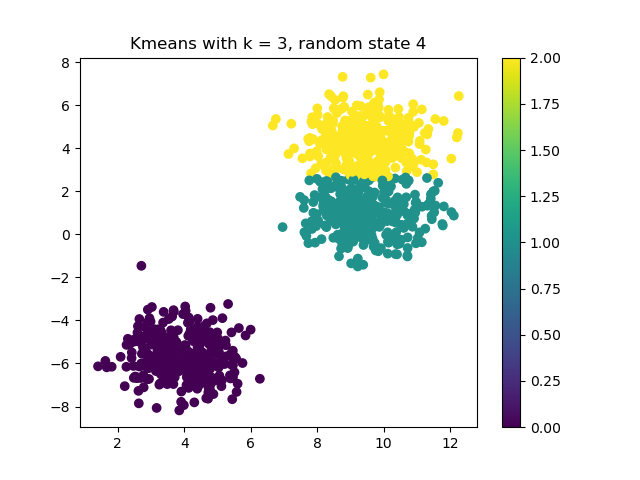
\includegraphics[scale=0.4]{images/task2_drs_rs4__k3}
    \end{minipage}
    \begin{minipage}{0.5\textwidth}
    \centering
    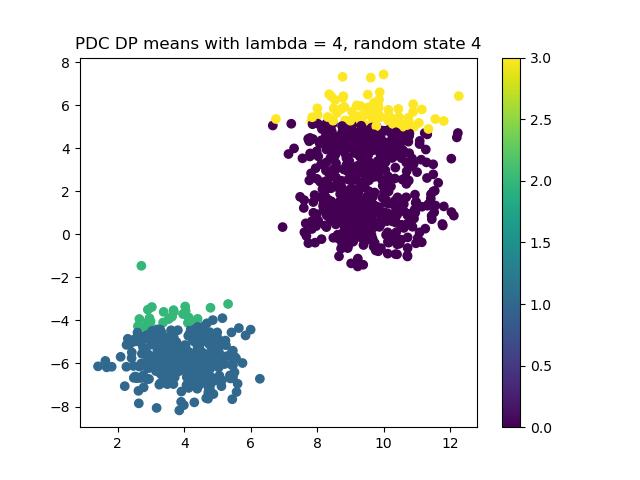
\includegraphics[scale=0.4]{images/task2_drs_rs4__l4}
    \end{minipage}
    \caption{Diffrent samples space initializations}\label{fig:figure4}
\end{figure}

Based on the figures above, both algorithms performed reasonably well on the datasets.
However, k-means seemed to perform slightly better in terms of producing visually distinct clusters with clear boundaries.
This is likely due to the choice of the lambda in dc-dp means,
which may have led to too many splits and resulting in the formation of more numerous, smaller clusters.
Either way the results demonstrate the different behavior of the two algorithms.
\pagebreak
\subsection*{Different hyper parameters}
Now we will test our algorithms on the same dataset, with different values for their respective hyper parameters.
\subsubsection*{Kmeans:}
\begin{figure}[!h]
    \begin{minipage}{0.5\textwidth}
    \centering
    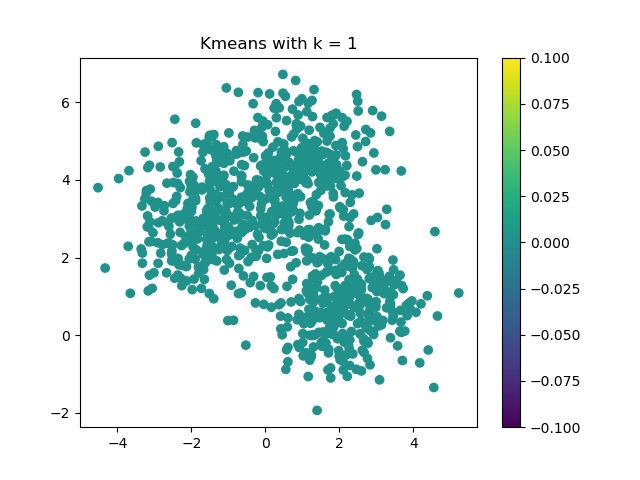
\includegraphics[scale=0.4]{images/task2_dkv__k1}
    \end{minipage}
    \begin{minipage}{0.5\textwidth}
    \centering
    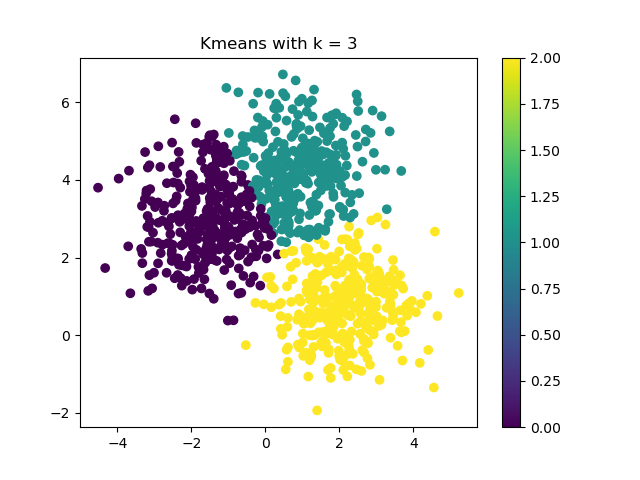
\includegraphics[scale=0.4]{images/task2_dkv__k3}
    \end{minipage}
    \begin{minipage}{0.5\textwidth}
    \centering
    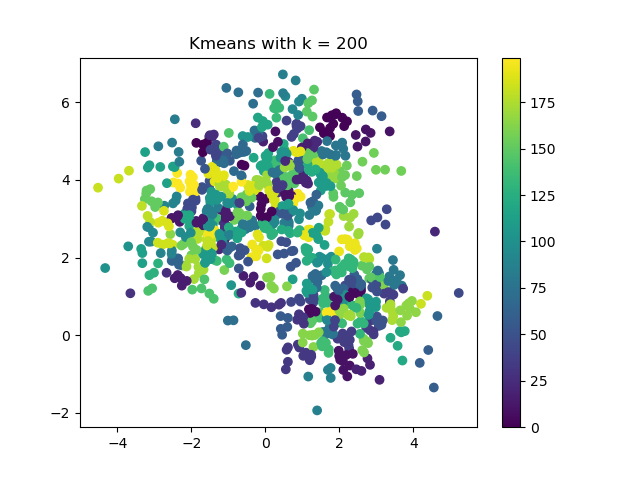
\includegraphics[scale=0.4]{images/task2_dkv__k200}
    \end{minipage}
    \begin{minipage}{0.5\textwidth}
    \centering
    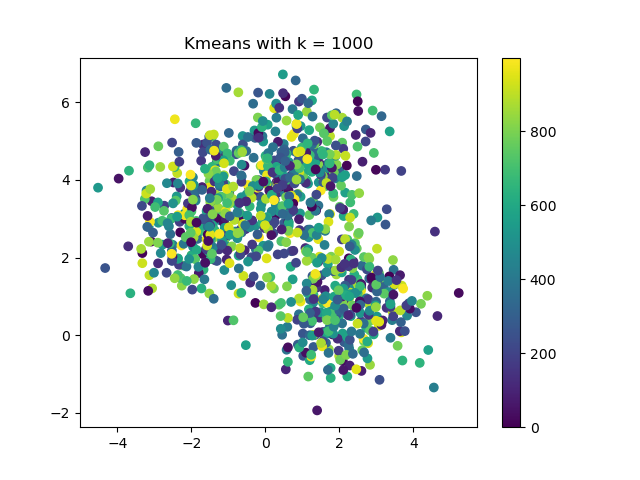
\includegraphics[scale=0.4]{images/task2_dkv__k1000}
    \end{minipage}
    \caption{Kmeans with different values of k}\label{fig:figure5}
\end{figure}

The initial experiment with k=1 resulted in all the samples being assigned to a single cluster, which is not useful for data analysis.
However, as the value of k was increased to 3, the algorithm produced a clustering result that appeared to be the most reasonable,
with distinct clusters formed around the data's structure.
As k was further increased, the number of clusters gradually increased,but the resulting clusters became less cohesive,
and the boundaries between them became blurred.
This highlights the trade-off between the number of clusters and the cohesiveness of the clusters, which is a
critical factor in choosing the optimal value of k for k-means clustering.
\pagebreak
\subsubsection*{DC-DP-Means:}
\begin{figure}[!h]
    \begin{minipage}{0.5\textwidth}
    \centering
    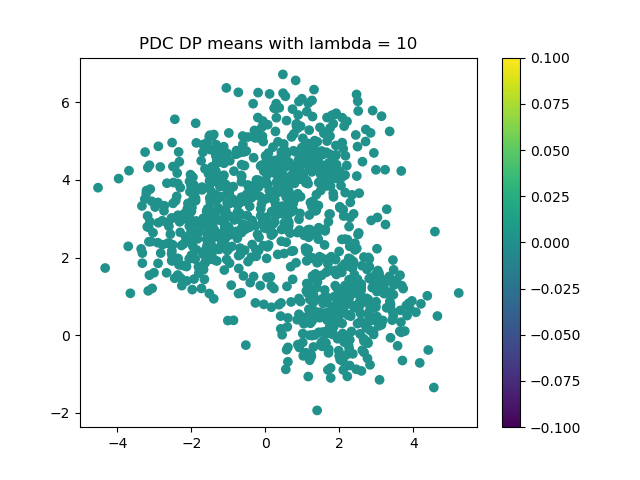
\includegraphics[scale=0.4]{images/task2_dlv__l10}
    \end{minipage}
    \begin{minipage}{0.5\textwidth}
    \centering
    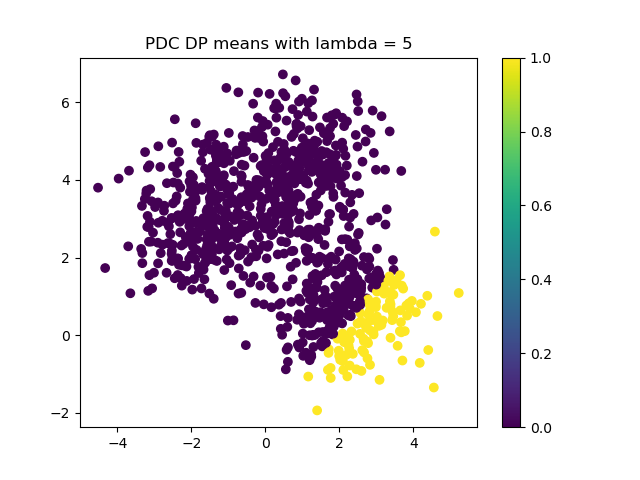
\includegraphics[scale=0.4]{images/task2_dlv__l5}
    \end{minipage}
    \begin{minipage}{0.5\textwidth}
    \centering
    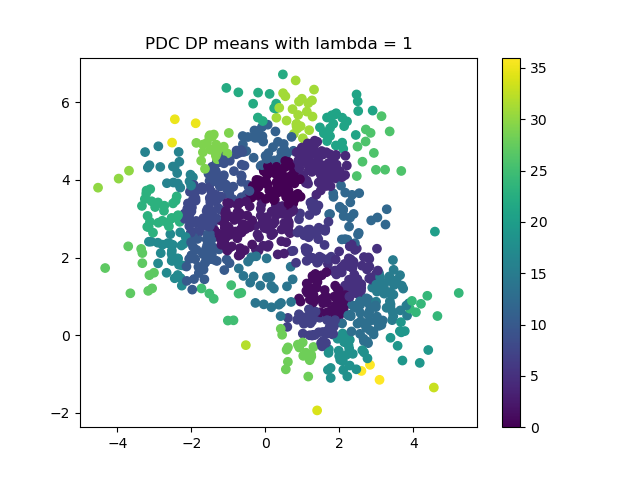
\includegraphics[scale=0.4]{images/task2_dlv__l1}
    \end{minipage}
    \begin{minipage}{0.5\textwidth}
    \centering
    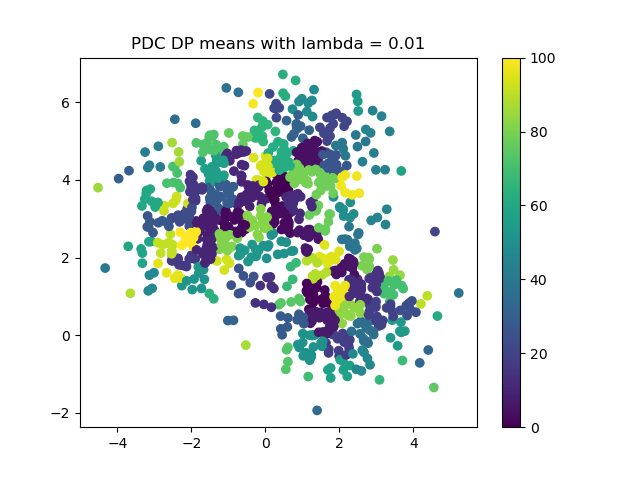
\includegraphics[scale=0.4]{images/task2_dlv__l0.01}
    \end{minipage}
    \caption{DC-DP-Means with different values of l}\label{fig:figure6}
\end{figure}
 We started with l=10, which produced a single cluster encompassing all the samples in the dataset this makes sense
 because l indicate the maximal distance between points in a cluster and 10 captures all the space.
 As we gradually decreased the value of l, the number of clusters increased, and the resulting clusters became more cohesive and distinct.
 Yet around 1 the number of clusters increased dramatically, and the clusters became less cohesive and more blurred.
 The best clustering result is probably when l is set between 2-4.
\pagebreak
\section*{Task 3}\label{sec:task-3}
Now we will apply the algorithms we have developed to a real-world dataset.
We have taken the following image of a mandrill monkey from the web and compressed it to reduce calculation time.
\begin{figure}[!h]
    \centering
    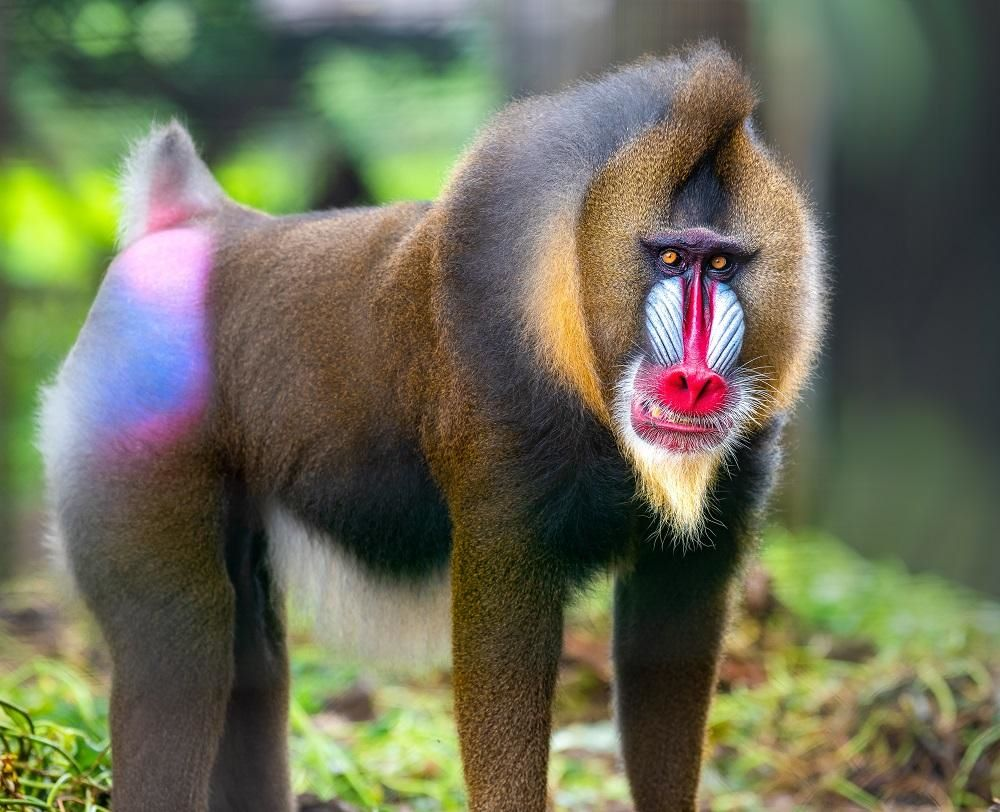
\includegraphics[scale=0.4]{images/monkey}
    \caption{Real image (scaled down)}
    \label{fig:real}
\end{figure}
\begin{figure}[!h]
    \centering
    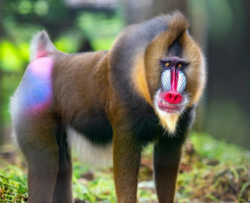
\includegraphics[]{images/monkey_compressed}
    \caption{Compressed image}
    \label{fig:compressed}
\end{figure}
\pagebreak
\subsection*{K-means:}
    \begin{figure}[!h]
        \begin{minipage}{0.5\textwidth}
        \centering
        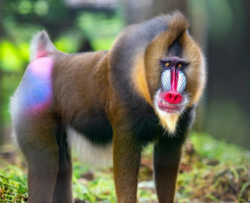
\includegraphics[]{images/monkey_compressed}
        \caption{Original}
        \end{minipage}
        \begin{minipage}{0.5\textwidth}
        \centering
        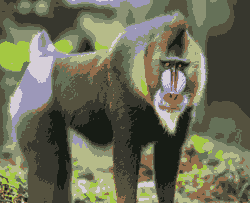
\includegraphics[]{images/monkey_clustered_kmeans_k_10}
        \caption{k = 10}
        \end{minipage}
        \begin{minipage}{0.5\textwidth}
        \centering
        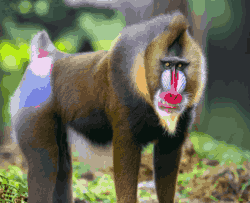
\includegraphics[]{images/monkey_clustered_kmeans_k_50}
        \caption{k = 50}
        \end{minipage}
        \begin{minipage}{0.5\textwidth}
        \centering
        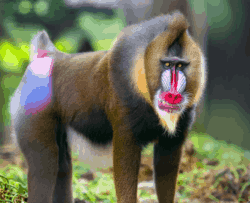
\includegraphics[]{images/monkey_clustered_kmeans_k_100}
        \caption{k = 100}
        \end{minipage}\label{fig:figure7}
	\end{figure}
    As seen above, when choosing k=10, the algorithm produced a clustering result that appears lacking in the distinctiveness of the mandrill's colors.
    This is expected, as 10 colors is not enough to capture the full range of colors in the image.
    As k was increased to 50, the resulting clusters became more cohesive and distinct, and the colors and structure of the mandrill became more apparent.
    At k=100 we get a pretty good clustering result, looking almost identical to the original image at most places.
    \pagebreak
    \subsection*{DC-DP-Means:}
        \begin{figure}[!h]
        \begin{minipage}{0.5\textwidth}
        \centering
        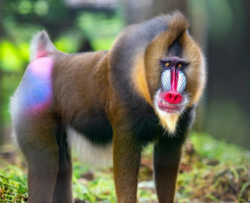
\includegraphics[]{images/monkey_compressed}
        \caption{Original}
        \end{minipage}
        \begin{minipage}{0.5\textwidth}
        \centering
        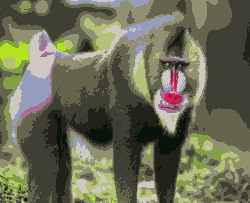
\includegraphics[]{images/monkey_clustered_pdc_dp_means_l_100}
        \caption{l = 100}
        \end{minipage}
        \begin{minipage}{0.5\textwidth}
        \centering
        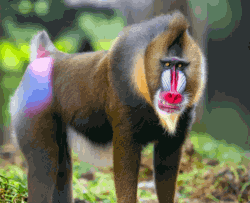
\includegraphics[]{images/monkey_clustered_pdc_dp_means_l_20}
        \caption{l = 20}
        \end{minipage}
        \begin{minipage}{0.5\textwidth}
        \centering
        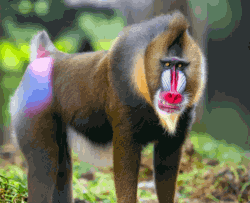
\includegraphics[]{images/monkey_clustered_pdc_dp_means_l_5}
        \caption{l = 5}
        \end{minipage}\label{fig:figure8}
	\end{figure}
    As seen above, when choosing l=100, the algorithm produced a clustering result that appears lacking like when we chose k = 10.
    This is also expected, as 100 is a large distance required to split a cluster, therefore we end up with a few large clusters.
    As l was decreased to 20, the results improved dramatically, and the colors and structure of the mandrill became more apparent.
    decreasing l further to 5 didn't seem to improve much on the already impressive result.
\end{document}